\documentclass[tikz]{standalone}

\usepackage{tikz}
\usetikzlibrary{positioning}

\begin{document}

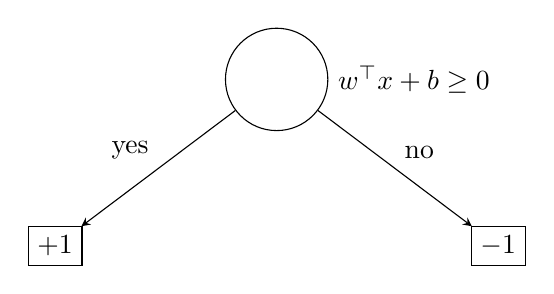
\begin{tikzpicture}[>=stealth, node distance=1.8cm]
    % root node
    \node[circle,draw,minimum width=13mm,label=right:{$w^\top x + b \ge 0$}] (root) {};

    % leaves
    \node[draw,rectangle,below left=1.4cm and 2.0cm of root]  (plus)  {$+1$};
    \node[draw,rectangle,below right=1.4cm and 2.0cm of root] (minus) {$-1$};

    % edges
    \draw[->] (root) -- node[above left]  {yes} (plus);
    \draw[->] (root) -- node[above right] {no}  (minus);
\end{tikzpicture}

\end{document}